\documentclass{IEEEtran}
\usepackage[pdftex]{graphicx}
\usepackage{cite}
\newcommand{\HRule}{\rule{\linewidth}{0.5mm}}
\usepackage{color}
\usepackage{listings}
\definecolor{mygreen}{rgb}{0,0.6,0}
\definecolor{mygray}{rgb}{0.9,0.9,0.9}
\definecolor{mymauve}{rgb}{0.58,0,0.52}
\lstset{
  backgroundcolor=\color{mygray},     % choose the background color; you must add \usepackage{color} or \usepackage{xcolor}
  basicstyle=\tiny\ttfamily,  % the size of the fonts that are used for the code
  breakatwhitespace=false,            % sets if automatic breaks should only happen at whitespace
  breaklines=true,                    % sets automatic line breaking
  captionpos=b,                       % sets the caption-position to bottom
  commentstyle=\color{mygreen},       % comment style
  deletekeywords={...},               % if you want to delete keywords from the given language
  escapeinside={\%*}{*)},             % if you want to add LaTeX within your code
  extendedchars=true,                 % lets you use non-ASCII characters; for 8-bits encodings only, does not work with UTF-8
  frame=single,                       % adds a frame around the code
  keepspaces=true,                    % keeps spaces in text, useful for keeping indentation of code (possibly needs columns=flexible)
  keywordstyle=\color{blue},          % keyword style
  language=Verilog,                   % the language of the code
  morekeywords={*,...},               % if you want to add more keywords to the set
  numbers=left,                       % where to put the line-numbers; possible values are (none, left, right)
  numbersep=5pt,                      % how far the line-numbers are from the code
  numberstyle=\tiny\color{mygray},    % the style that is used for the line-numbers
  rulecolor=\color{black},            % if not set, the frame-color may be changed on line-breaks within not-black text (e.g. comments (green here))
  showspaces=false,                   % show spaces everywhere adding particular underscores; it overrides 'showstringspaces'
  showstringspaces=false,             % underline spaces within strings only
  showtabs=false,                     % show tabs within strings adding particular underscores
  stepnumber=2,                       % the step between two line-numbers. If it's 1, each line will be numbered
  stringstyle=\color{mymauve},        % string literal style
  tabsize=1,                          % sets default tabsize to 2 spaces
  %title=\lstname                      % show the filename of files included with \lstinputlisting; also try caption instead of title
}

\begin{document}
\begin{titlepage}
\begin{center}

% Upper part of the page. The '~' is needed because \\
% only works if a paragraph has started.
%\includegraphics[width=0.15\textwidth]{./logo}~\\[1cm]

\textsc{\LARGE CSU Sacramento}\\[1.5cm]

\textsc{\Large EEE 184: Intro to Feedback Systems}\\[0.5cm]

% Title
\HRule \\[0.4cm]
{ \huge \bfseries Two Axis Gimbal \\[0.4cm] }

\HRule \\[1.5cm]

% Author and supervisor
\begin{minipage}{0.4\textwidth}
\begin{flushleft} \large
\emph{Author:}\\
Curtis \textsc{Muntz}\\
David \textsc{Larribas}\\
Michael \textsc{Frith}
\end{flushleft}
\end{minipage}
\begin{minipage}{0.4\textwidth}
\begin{flushright} \large
\emph{Instructor:} \\
Dr. \textsc{Belkhouche}
\end{flushright}
\end{minipage}

\vfill

% Bottom of the page
{\large \today}

\end{center}
\end{titlepage}
\vfill

\begin{abstract}
A 2-axis gimbal controlled by an Arduino Uno microcontroller. The angle is determined by an IMU sensor which provides accelerometer and gyroscope data. The microcontroller processes this data using a complementary filter. A Taylor series approximation is used to determine the angle accurately up to $30^\circ$. This system uses the feedback from the sensors in an attempt to stabilize itself to the angles read.
\end{abstract}

\section{Intro}
We are tasked with building a project that takes a sensor, a microcontroller, and an actuator to create a control system. We decided to build a 2-axis gimbal, a device that keeps a camera's attitude nominally consistent in the chosen axes regardless of its mounted system. If a gimbal is attached to a multi rotor helicopter, it will keep the camera level independent of the pitch and roll of the airframe.



\section{Physical Setup}

To control the camera in the two axes, two servo motors are used; one per axis. They are connected on a metal frame as pictured in Figure \ref{physicalPIC}. The microcontroller processes the data from the IMU and converts this into a PWM that the servos can understand. The motors are controlled by PWM signals sent to it from the microcontroller. An Arduino Uno microcontroller is being used for this project because it was already owned and possesses enough processing power to process the sensor data and control the motors. The gyroscope and accelerometer are located on an MPU 6050 IMU (inertial measurement unit) with a GY-521 breakout. The IMU is located on a breadboard that is mounted on the gimbal handle. Two 9-volt batteries in parallel are fed into a LM7805 linear voltage regulator to convert the voltage to 5V which supplies the power to every component making the unit self contained. A USB port is also attached to the board as a means to supply power to the Arduino without the need to connect to a computer to run or power the systems.

\begin{figure}[ht!]
    \centering
    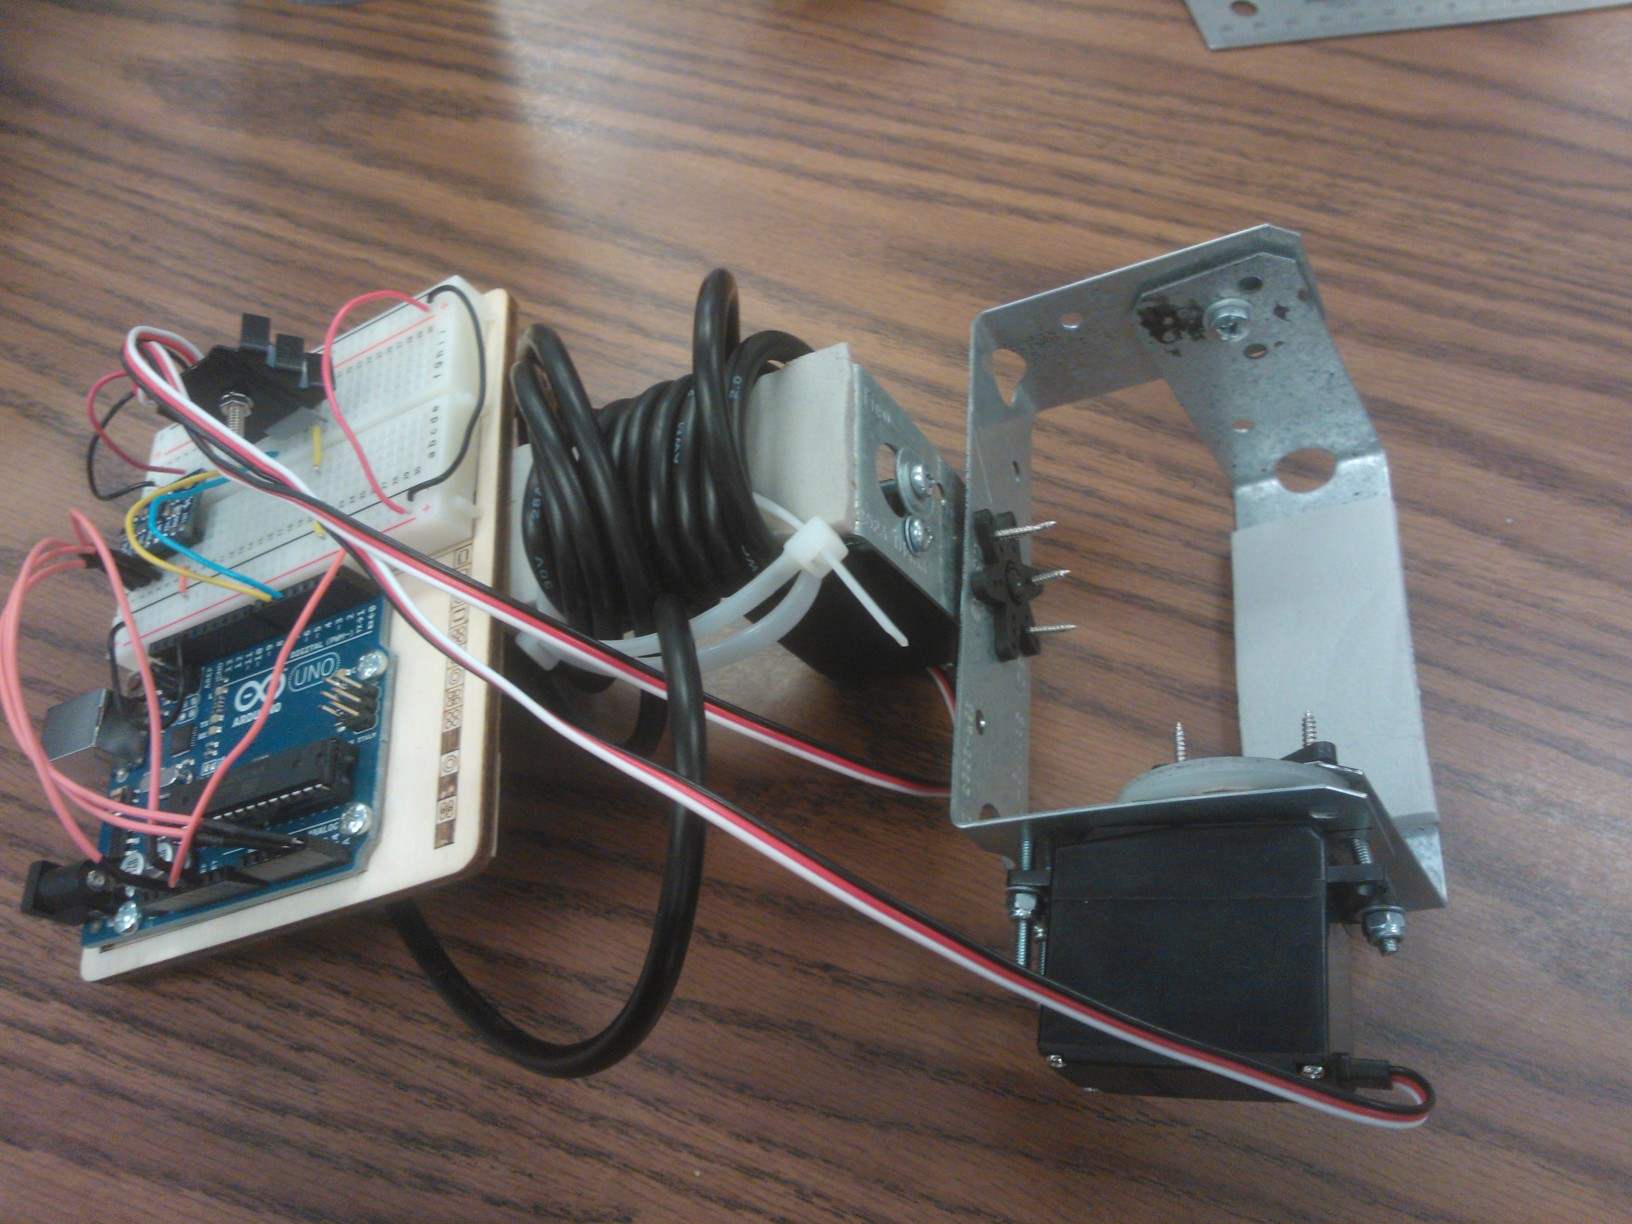
\includegraphics[width=0.4\textwidth]{physical}
    \caption{\emph{Physical Layout}}
    \label{physicalPIC}
\end{figure}


\section{Gyro Data}
After initially calibrating the IMU, the gyroscope data was analyzed. Because gyroscopes measure the angular rotation about an axis, it is simplest to estimate any change in angle experienced by the IMU by integrating the resultant data. We can find the angle $\theta$ using Equation \ref{gyro} below where $\dot{\theta}$ is the gyroscope's measured rate of angular change.


\begin{equation} 
\label{gyro}
\theta=\int{\dot{\theta}}dt
\end{equation}

This implies that if we know the sampling rate of the IMU, and the value of rotation/s, we can discern an angle to which the IMU has rotated. The integral is approximated by summing the previous angle with the change in angle; however, there is a problem with using only the gyroscope data. Because of circuit limitations, such as internal clocks, we cannot guarantee the exact change from the initial cycle to the next cycle. We can only discern the change over that period of time. Because of this, there is a slight error assumed every time we integrate the angle rate. Since this resultant angle is fed back into the input of the gyroscope angle approximation function, this error continuously adds onto itself and eventually becomes very significant. This concept is known as gyroscopic drift. After a certain amount of time, depending on the gyroscope and sensitivity of measurements, the data returned from the gyroscope is essentially unusable.

The gyroscope angle estimation was realized in code by:
\begin{lstlisting}[language=C++]{Name=gyro}
/*
Takes in raw data, multiplies by scalar and sample time to get angular rate, and adds to previous angle, where gx is the gyroscope data.
*/
  xGyro_raw = gx - xGyro_calibrate;
  xGyro_rate = (xGyro_raw * xGyro_scale) * gyro_time;
  xGyro_angle += xGyro_rate;
\end{lstlisting}


\section{Accelerometer Data}
In order to fix the gyroscope drift, accelerometer data was included as a form of reality check.

The reason we don't use accelerometer data for the initial control scheme and instead chose to use the gyroscope data because accelerometers are sensitive to noise. In particular, the accelerometer is sensitive to self-inflicted noise. For example when using a servo or motor, any movement performed by the motors can induce a torque into the physical frame, which will affect the reading of the accelerometer

The data returned by the accelerometer is split into three values corresponding to the three planar axes: $A_x$, $A_y$, and $A_z$. These values are all interrelated, as they essentially answer the question ``how is gravity affecting me?'' The answer to this question relies a bit of trigonometry.


\begin{figure}[ht!]
  \centering
      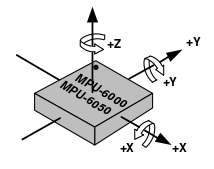
\includegraphics[width=0.4\textwidth]{orientation}
  \caption{\emph{Orientation of Axes of Sensitivity and Polarity of Rotation \cite{mpuPSmanual}}}

\end{figure}


\section{Linearization}
The three accelerometers return nominal values between -2000 and 2000 on their axis's extremities. This means with no additional forces and the accelerometer tilted to the maximum reading and not in motion, the value read is either -2000 or 2000, depending on its orientation. The angle associated with these values are -90 and +90 degrees. A simple mapping could be used to translate these values to resolve an angle, however, we are utilizing the arcsine function to achieve the angle from our obtained value. 

We are able to use arcsine as means to measure the angle if and only if the device is held stationary. This gives us a reference vector of $1 g$ pointed straight down due to gravity. As we tilt the device along the x or y axis, the accelerometer measures the distance along the x and y axis that the gravity vector sweeps in that direction as it tilts. As the angle to that swept distance is opposite of the created length (accelerometer value) and the hypotenuse length is 1 proportionately to gravity, we can use that swept length over the hypotenuse length of 1 to give us an angle utilizing arcsin.


However, arcsine is fairly nonlinear. In order to get a linear value mapping, we must use a linearized region of the arcsine function. Using the Taylor series expansion of arcsine, the first term is x. Fortunately, for small angles (below 30 degrees) this holds to be highly linear.  We procured a protractor and measured the value of the accelerometers at +/-30 degrees off their respective angle of measure and obtained values from the accelerometers of +/-1000, respectively.

\begin{equation}
\label{taylor}
\sin^{-1}(x)=x+\frac{x^3}{6}+\frac{x^5}{40}+\ldots
\end{equation}



We can now map our angles to values received from the accelerometer, which will hold accurate as long as we stay within +/- 45 degrees or so off their axes. As 30 degrees resulted in a value of 1000, 1 degree will result in a value of approximately 30. If we receive a value from our accelerometer, we can multiply by the inverse of this relationship and obtain the small angle approximation after linearization.

The accelerometer angle estimation was realized in code by:
\begin{lstlisting}[language=C++]{Name=gyro}
/*
Reads ay from the accelerometer. The 30 is our scalar that achieves linearization.
*/
    xAccel_raw = (float) ay/30;
\end{lstlisting}

\section{Filtering}
Now that gyroscope and accelerometer angles have been resolved, we realize a filtered angle using a complementary filter. Equation \ref{filter} shows the complementary filter. This essentially sets up a high pass filter for the gyroscope, as it will be our main source of data, and sets up a low pass filter for the accelerometer in order to reduce the the effect of noise.

\begin{equation} 
\label{filter}
\theta_{total} = (G * 0.95) + (A * 0.05)
\end{equation}

The resulting angle is sufficiently suitable for our interests. Figure 3 compares the data returned by the gyro alone, the accelerometer alone, and the complementary filter. Note that the drift is eliminated, and the noise of the accelerometer is not translated into the filtered angle.


\begin{figure}[ht!]
\centering
\label{chart2}
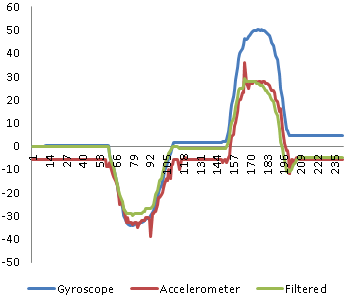
\includegraphics[width=0.4\textwidth]{david}
\caption{\emph{Filtered Data}}
\end{figure}


\section{Controlling Servo Orientation}
Now that we have an angle detection filter working properly, we can implement a servo control algorithm that compensates for the movement of the servos. By subtracting the change from the original angle, we write the resulting answer to the servos using the built in Arduino servo library. Any deviation away from the nominal origin would be compensated by writing the opposite angle to the servo corresponding to that axis.

\section{Conclusions}
The servos respond to the tilt of the IMU in the directions intended to keep the camera stable, but the system is not as stable as we would like it to be. There is a significant amount of jitter, but this is mostly due to the thin metal frame. When the servos stop abruptly, the frame oscillates rapidly, which adds unwanted motion to the camera's image and adds error to the accelerometer. Also, the frame was not balanced and this is causing the servos to work harder which drains the batteries more and results in a less efficient system. Updating the frame to a more stable wood or plastic material and adding counterweights would lessen much of the instability. The frame is also built in such a way that its bolts infringe its movement. Updating the frame should fix this too. Lessening the weight of the servos and system as a whole would decrease the jitter and make the system easier to handle. 
In addition to these physical changes, the code can be taken far beyond where it is now in complexity which could immensely increase the accuracy of the system, but for the scope of the project, the gimbal stabilizes itself well.

\begin{thebibliography}{9}

\bibitem{mpuPSmanual}
      % Leslie Lamport,
      % \emph{\LaTeX: A Document Preparation System},
      % Addison Wesley, Massachusetts,
      % 2nd Edition,
      % 1994.

    InvenSense
    \emph{MPU 6050},
    http://invensense.com/mems/gyro/documents/ PS-MPU-6000A-00v3.4.pdf,
        page 40,
    2013.


\bibitem{filterspdf}
         MIT,
    \emph{The Balance Filter},
    http://web.mit.edu/scolton/www/filter.pdf,
    2007.

\bibitem{jeffrowberg}
Jeff Rowberg,
\emph{i2c Development Library},
    https://github.com/jrowberg/i2cdevlib/tree/ master/Arduino/MPU6050,
    2013.

\bibitem{arduinoRobotics}
    JD Warren,
    \emph{Arduino Robotics},
    Apress,
    1st Edition,
    2011.
 
@Article{Hunter:2007,
  Author    = {Hunter, J. D.},
  Title     = {Matplotlib: A 2D graphics environment},
  Journal   = {Computing In Science \& Engineering},
  Volume    = {9},
  Number    = {3},
  Pages     = {90--95},
  abstract  = {Matplotlib is a 2D graphics package used for Python
  for application development, interactive scripting, and
  publication-quality image generation across user
  interfaces and operating systems.},
  publisher = {IEEE COMPUTER SOC},
  year      = 2007
}

\end{thebibliography}

\end{document}



